\section{Luthfi Muhammad Nabil (1174035)}
\subsection{Point Poly}
\begin{enumerate}
    \item Nomor 1
    \lstinputlisting{src/1/1174035/tugas2/praktek1_pyshp.py}
    \begin{figure}[H]
		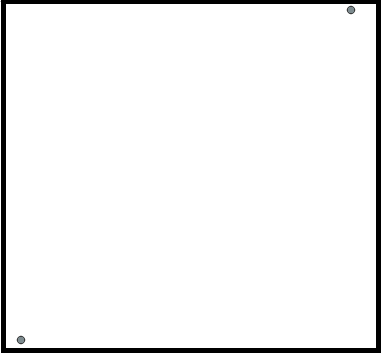
\includegraphics[width=6cm]{figures/1174035/tugas2/soal_1.png}
		\centering
		\caption{Nomor 1}
	\end{figure}
    \item Nomor 2
    \lstinputlisting{src/1/1174035/tugas2/praktek2_pyshp.py}
    \begin{figure}[H]
		
\includegraphics[width=6cm]{figures/1174035/tugas2/soal_2.png}
		\centering
		\caption{Nomor 2}
	\end{figure}
    \item Nomor 3
    \lstinputlisting{src/1/1174035/tugas2/praktek3_pyshp.py}
    \begin{figure}[H]
		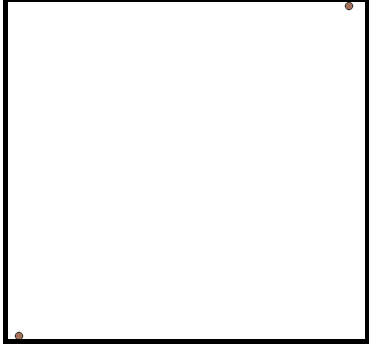
\includegraphics[width=6cm]{figures/1174035/tugas2/soal_3.png}
		\centering
		\caption{Nomor 3}
	\end{figure}
    \item Nomor 4
    \lstinputlisting{src/1/1174035/tugas2/praktek4_pyshp.py}
    \begin{figure}[H]
		
\includegraphics[width=6cm]{figures/1174035/tugas2/soal_4.png}
		\centering
		\caption{Nomor 4}
	\end{figure}
    \item Nomor 5
    \lstinputlisting{src/1/1174035/tugas2/praktek5_pyshp.py}
    \begin{figure}[H]
		
\includegraphics[width=6cm]{figures/1174035/tugas2/soal_5.png}
		\centering
		\caption{Nomor 5}
	\end{figure}
    \item Nomor 6
    \lstinputlisting{src/1/1174035/tugas2/praktek6_pyshp.py}
    \begin{figure}[H]
		
\includegraphics[width=6cm]{figures/1174035/tugas2/soal_6.png}
		\centering
		\caption{Nomor 6}
	\end{figure}
    \item Nomor 7
    \lstinputlisting{src/1/1174035/tugas2/praktek7_pyshp.py}
    \begin{figure}[H]
		
\includegraphics[width=6cm]{figures/1174035/tugas2/soal_7.png}
		\centering
		\caption{Nomor 7}
	\end{figure}
    \item Nomor 8
    \lstinputlisting{src/1/1174035/tugas2/praktek8_pyshp.py}
    \begin{figure}[H]
		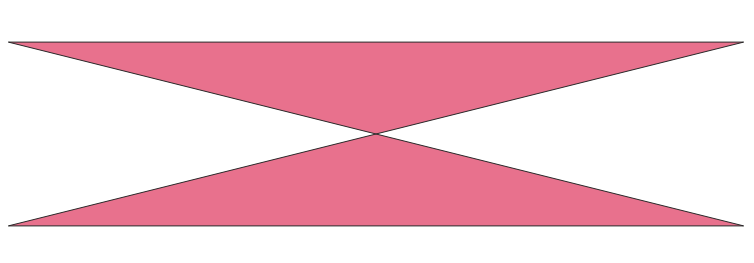
\includegraphics[width=6cm]{figures/1174035/tugas2/soal_8.png}
		\centering
		\caption{Nomor 8}
	\end{figure}
    \item Nomor 9
    \lstinputlisting{src/1/1174035/tugas2/praktek9_pyshp.py}
    \begin{figure}[H]
		
\includegraphics[width=6cm]{figures/1174035/tugas2/soal_9.png}
		\centering
		\caption{Nomor 9}
	\end{figure}
    \item Nomor 10
    \lstinputlisting{src/1/1174035/tugas2/praktek10_pyshp.py}
    \begin{figure}[H]
		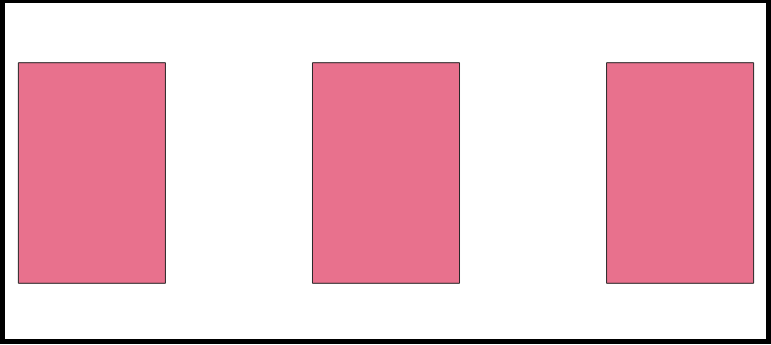
\includegraphics[width=6cm]{figures/1174035/tugas2/soal_10.png}
		\centering
		\caption{Nomor 10}
	\end{figure}
\end{enumerate}
\subsection{Link Youtube}